\section{Connected Components Labeling}
\writtenby{\dcauthornameewie}%
Um zusammenhängende Bildstrukturen zu erfassen verwendet man dass sogenannte Connected Components Labeling.
Dabei wird jeder Bildpunkt genau einer Menge zugeordnet welche je eine Komponente zusammenhängenger Bildpunkte repräsentiert.
Zwei Bildpunkte hängen zusammen, wenn diese benachbart sind und den gleichen Wert besitzen.
Für die Nachbarschaft gibt es verschiedene Modelle.
%
\begin{description}
\item[4-Konnektivität] betrachtet für ein Pixel $(x,y)$ die 4 Pixel $(x\pm1,y)$ und $(x,y\pm1)$
\item[8-Konnektivität] betrachtet für ein Pixel $(x,y)$ neben den 4 Pixel der 4-Konnektivität zusätzlich noch die 4 Pixel $(x\pm1,y\pm1)$
\end{description}
%
\begin{figure}[H]
  \centering
  \begin{subfigure}{0.3\columnwidth}
    \centering
    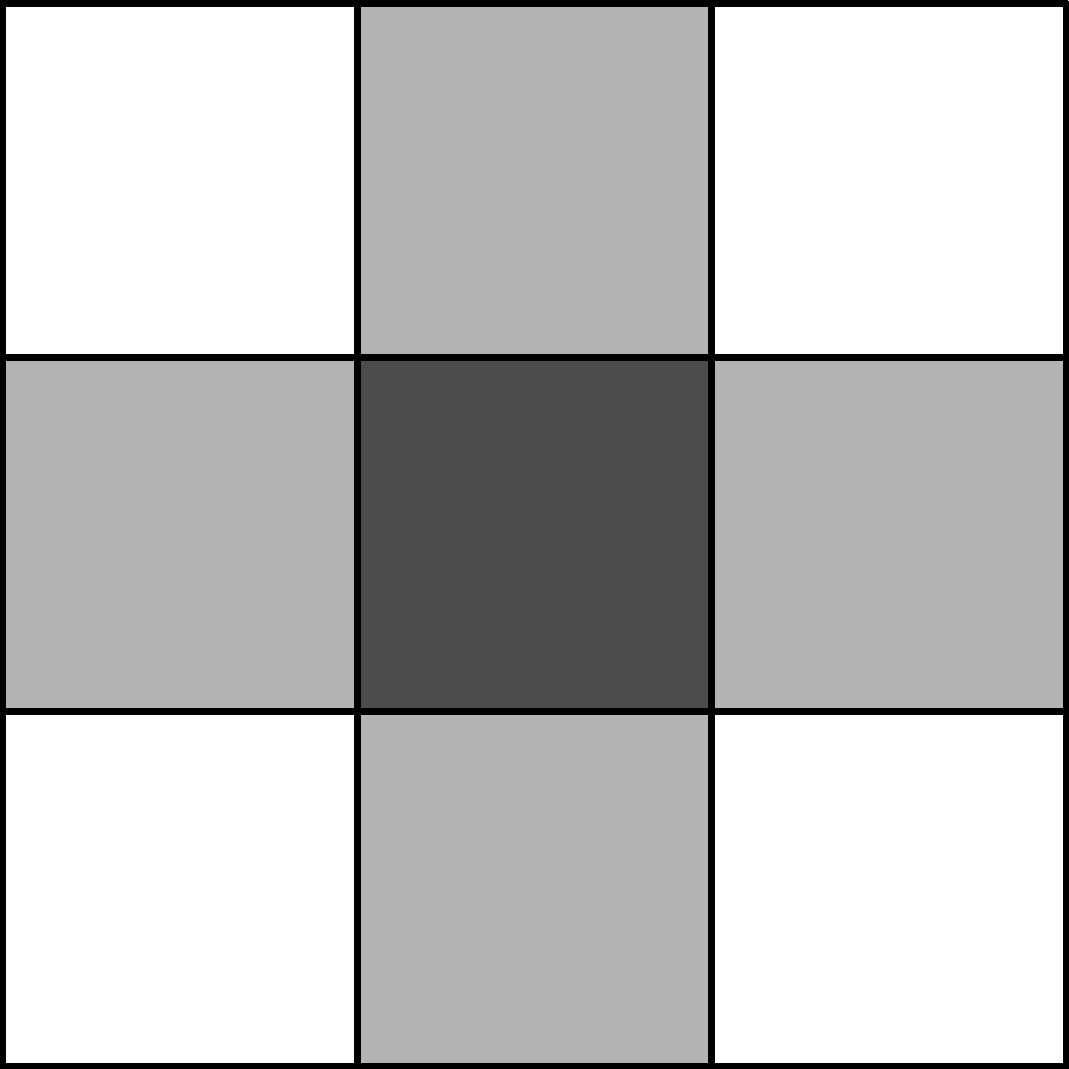
\includegraphics[width=0.5\columnwidth]{img/basics/connected-compontents/4-connectivity}
    \caption{4-Konnektivität}
  \end{subfigure}
  \begin{subfigure}{0.3\columnwidth}
    \centering
    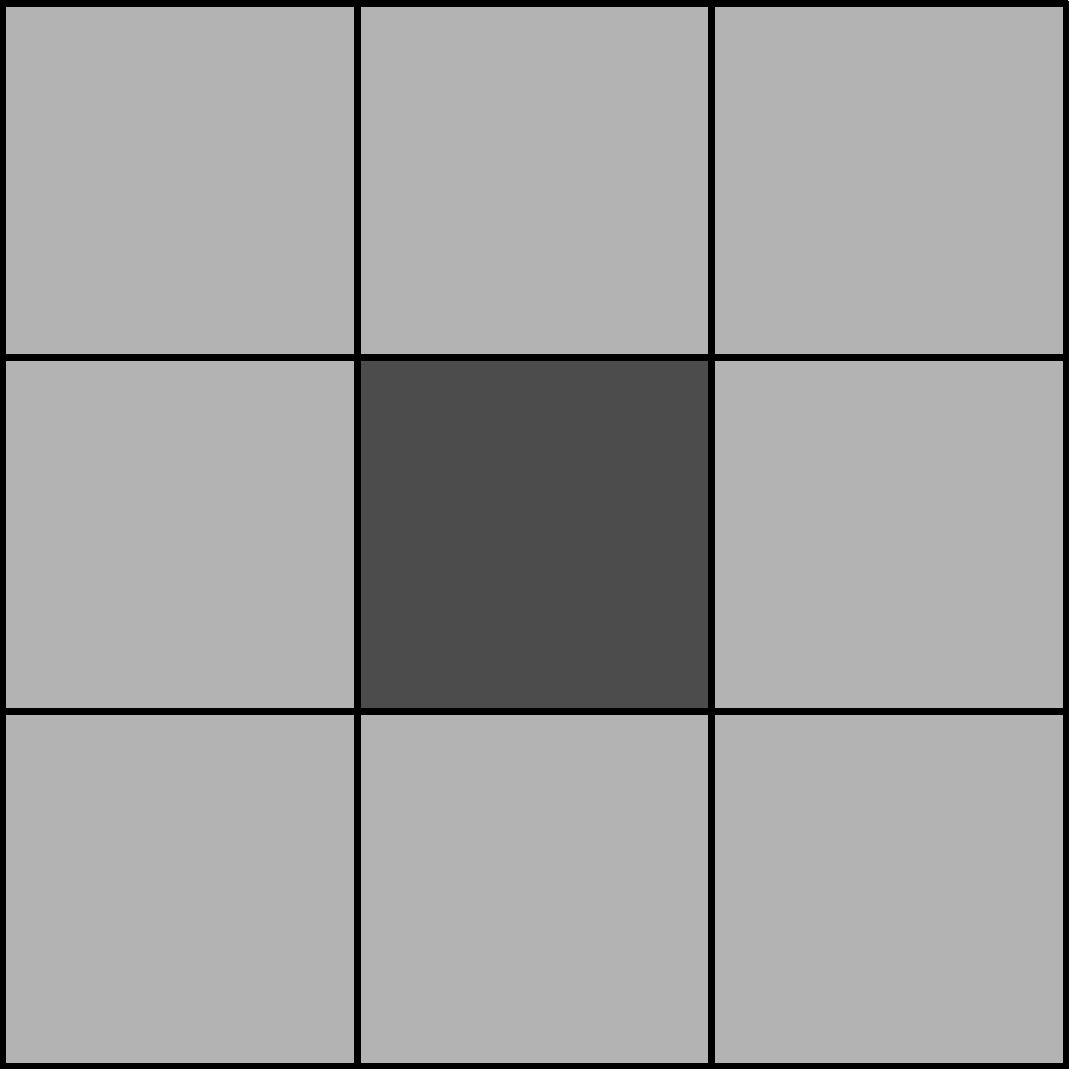
\includegraphics[width=0.5\columnwidth]{img/basics/connected-compontents/8-connectivity}
    \caption{8-Konnektivität}
  \end{subfigure}
  \caption[Vergleich von Pixelnachbarschaften]{Vergleich von Pixelnachbarschaften, mit dem betrachteten Pixel markiert in Dunkelgrau und den Pixeln der Nachbarschaft in Hellgrau.}
\end{figure}
%
Je mehr Pixel als Nachbarschaft herangezogen werden, desto größer können die zusammenhängenden Komponenten ausfallen, da es mehr Möglichkeiten gibt in denen zwei Pixel als verbunden gelten.

Das Connected Component Labeling ist realisierbar mittels eines Scanlineverfahrens \cite[S.~69--75]{compvis2001}, d.h. jede Bildzeile wird, mit der oberen Zeile ($y=0$) beginnend, pixelweise von links ($x=0$) nach rechts verarbeitet.
Jedes Pixel wird auf Verbundenheit mit seinen Nachbarn (4-Konnektivität) oberhalb ($y-1$) und links ($x-1$) geprüft.
Unterscheidet sich der Wert des aktuellen Pixels von den betrachteten Nachbarn so wird diesem ein neues Label zugewiesen.
Besitzt das Pixel hingegen den Wert mindestens eines Nachbarn so wird das Label des Nachbarn zugewiesen.
Besitzen mehrere Nachbarn den gleichen Wert aber unterschiedliche Label, so werden diese Label als äquivalent markiert.
Die erste Bildzeile und -spalte müssen gesondert initialisert werden, da diese keine Nachbarn oberhalb bzw. links besitzen.
Sind alle Pixel verarbeitet, müssen Labeläquivalenzen aufgelöst werden, sodass Pixeln mit äquivalenten Label ein gemeinsames Label zugewiesen werden kann. Zum Erfassen der Äquivalenzen eignet sich die \emph{UnionFind} Datenstruktur.
